\documentclass[unicode,11pt,a4paper,oneside,numbers=endperiod,openany]{scrartcl}

\renewcommand{\thesubsection}{\arabic{subsection}}

\usepackage{graphicx}
\usepackage{longtable}
\usepackage{booktabs}
\usepackage{multirow}

\input{assignment.sty}


\begin{document}


\setassignment
\setduedate{Monday, 19 December 2024, 06:00 PM}

\serieheader{Experimentation and Evaluation}{2024}{\textbf{Students:} Davide Frova, Costanza Rodriguez Gavazzi}{}{Project 2}{}
\newline


\section{Abstract}
 

\section{Introduction}

Introduce the topic of investigation to the reader and motivate why you did the experiment.

\subsection{Hypotheses}
\textbf{Null Hypothesis}: There is no significant difference in reading speed between camelCase and kebab-case. \\
\hfill \\
\textbf{Alternative Hypothesis}: Users perform better with kebab-case compared to camelCase.

\section{Method}

\subsection{Variables}
\subsubsection{Independent Variable} 
\textbf{Case Style}: camelCase, kebab-case

\subsubsection{Dependent Variables}
\textbf{Response Time}: in milliseconds; \\
\textbf{Correctness}: true/false

\subsubsection{Control Variables}
Same questions presented in random order.

\subsubsection{Blocking Variable}
\textbf{Previous programming experience}: true/false.

\subsection{Design}
Single-Factor Experiment \\
\hfill \\
Within-Subject Design: Participants experienced both case styles in random order to reduce bias \\
\hfill \\
\begin{figure}[h]
    \centering
    \includegraphics[width=0.7\textwidth]{./figures/graph.pdf}
    \caption{Design of the experiment}
    \label{fig:graph}
\end{figure}

\subsection{Participants}
Total participant: 36 \\
\hfill \\
Age range:  \\
Programming experience: n participants 

\subsection{Apparatus and Materials}
Web app built with Next.js, React, and TypeScript, deployed on Vercel. //todo davide

\subsection{Procedure}
Participants:
\begin{itemize}
    \item Provided their age and if they had programming background.
    \item Completed a warm-up tutorial.
    \item Answered 10 camelCase and 10 kebab-case questions, randomly shuffled.
\end{itemize}
Recorded data included response times, correctness, age of participant and programming background.

\section{Results}
\subsection{Visual Overview}

\begin{figure}
    \centering
    \begin{minipage}{0.45\textwidth}
        \centering
        \includegraphics[width=\textwidth]{./figures/correct_camel_distr.png}
        \caption{Distribution of Correct Answers for camelCase}
        \label{fig:correct_camel_distr}
    \end{minipage}
    \hfill
    \begin{minipage}{0.45\textwidth}
        \centering
        \includegraphics[width=\textwidth]{./figures/correct_kebab_distr.png}
        \caption{Distribution of Correct Answers for kebab-case}
        \label{fig:correct_kebab_distr}
    \end{minipage}
\end{figure}

\begin{figure}[h!]
    \centering
    \begin{minipage}{0.45\textwidth}
        \centering
        \includegraphics[width=\textwidth]{./figures/correct_camel_noback.png}
        \caption{Correct Answers for camelCase with No Programming Background}
        \label{fig:correct_camel_noback}
    \end{minipage}
    \hfill
    \begin{minipage}{0.45\textwidth}
        \centering
        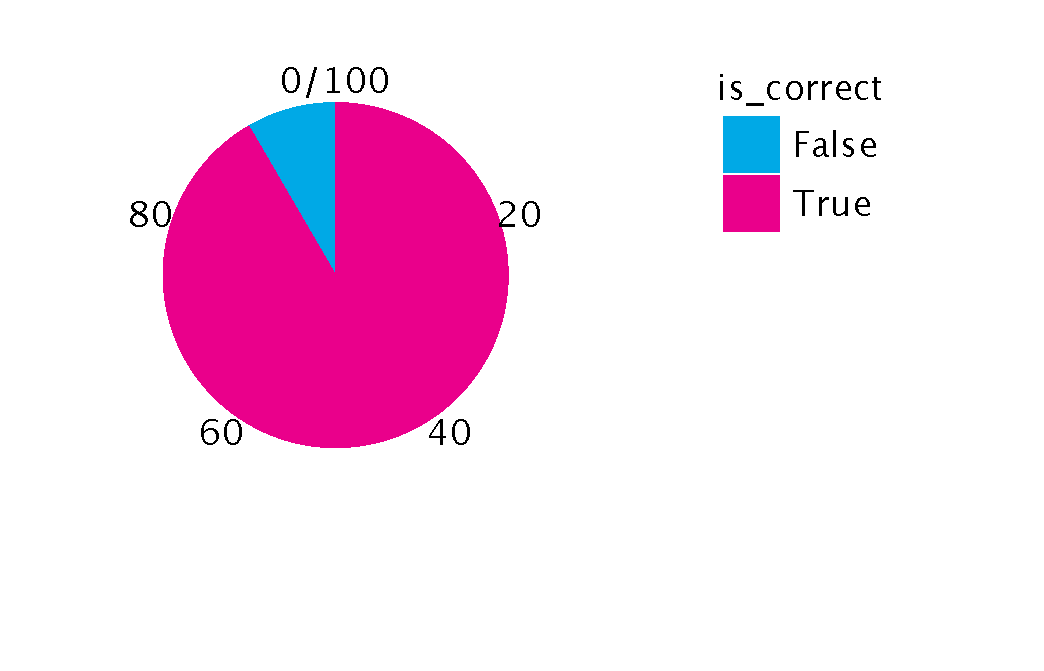
\includegraphics[width=\textwidth]{./figures/correct_camel_background.eps}
        \caption{Correct Answers for camelCase with Programming Background}
        \label{fig:correct_camel_background}
    \end{minipage}
    
    \vspace{0.5cm} 
    
    \begin{minipage}{0.45\textwidth}
        \centering
        \includegraphics[width=\textwidth]{./figures/correct_kebab_noBack.png}
        \caption{Correct Answers for kebab-case with No Programming Background}
        \label{fig:correct_kebab_noback}
    \end{minipage}
    \hfill
    \begin{minipage}{0.45\textwidth}
        \centering
        \includegraphics[width=\textwidth]{./figures/correct_keb_backgr.png}
        \caption{Correct Answers for kebab-case with Programming Background}
        \label{fig:correct_kebab_background}
    \end{minipage}
\end{figure}

\begin{figure}
    \centering
    \includegraphics[width=0.7\textwidth]{./figures/elapsed_time_correct.png}
    \caption{camelCase vs kebab-case: Elapsed Time}
    \label{fig:boxplot}
\end{figure}

\subsection{Descriptive Statistics}


\begin{table}[h]
    \centering
    \caption{Descriptive Statistics CSBG}
    \label{tab:descriptiveStatistics}
    {\resizebox{\textwidth}{!}{
            \begin{tabular}{lrrrrrrrr}
                \toprule
                              &            & Mean       & Std. Deviation & Minimum   & Maximum     & 25th percentile & 50th percentile & 75th percentile \\
                \cmidrule[0.4pt]{1-9}
                elapsed\_time & camelCase  & $3969.640$ & $2113.221$     & $150.000$ & $15059.000$ & $2548.250$      & $3511.000$      & $4987.750$      \\
                              & kebab-case & $4567.916$ & $3290.778$     & $328.000$ & $39951.000$ & $3007.250$      & $4007.500$      & $5118.750$      \\
                \bottomrule
            \end{tabular}
        }
    }
\end{table}

\begin{table}[h]
    \centering
    \caption{Descriptive Statistics NON CSBG}
    \label{tab:descriptiveStatistics}
    { \resizebox{\textwidth}{!}{
            \begin{tabular}{lrrrrrrrr}
                \toprule
                              &            & Mean       & Std. Deviation & Minimum    & Maximum     & 25th percentile & 50th percentile & 75th percentile \\
                \cmidrule[0.4pt]{1-9}
                elapsed\_time & camelCase  & $5296.818$ & $3376.998$     & $1744.000$ & $26341.000$ & $3200.250$      & $4419.500$      & $6334.250$      \\
                              & kebab-case & $6310.291$ & $4330.106$     & $1771.000$ & $31522.000$ & $3637.000$      & $4952.500$      & $7584.250$      \\
                \bottomrule
            \end{tabular}
        }}
\end{table}


\begin{table}[h]
    \centering
    \caption{Descriptive Statistics}
    \label{tab:descriptiveStatistics}
    \resizebox{\textwidth}{!}{
        \begin{tabular}{rrrrrrrr}
            \toprule
                       & Mean       & Std. Deviation & Minimum   & Maximum     & 25th percentile & 50th percentile & 75th percentile \\
            \cmidrule[0.4pt]{1-8}
            camelCase  & $4442.718$ & $2609.916$     & $150.000$ & $26341.000$ & $2734.000$      & $3904.000$      & $5522.000$      \\
            kebab-case & $5119.937$ & $3691.977$     & $497.000$ & $39951.000$ & $3209.500$      & $4319.000$      & $5624.000$      \\
            \bottomrule
        \end{tabular}
    }
\end{table}

\subsection{Inferential Statistics}

\begin{table}[h]
    \centering
    \caption{Paired Samples T-Test}
    \label{tab:pairedSamplesT-Test}
    {
        \begin{tabular}{lrrrrrrr}
            \toprule
            Measure 1  &   & Measure 2 & t       & df    & p       & Cohen's d & SE Cohen's d                                                             \\
            \cmidrule[0.4pt]{1-8}
            kebab-case & - & camelCase & $3.515$ & $359$ & $1.000$ & $0.185$   & $0.064$                                                                  \\
            \bottomrule
            \addlinespace[1ex]
            \multicolumn{8}{p{0.8\textwidth}}{\textit{Note.} For all tests, the alternative hypothesis specifies that kebab-case is less than camelCase.} \\
        \end{tabular}
    }
\end{table}


\section{Discussion}

\subsection{Compare Hypotheses with Results}
The null hypothesis is supported as no significant advantage was found for kebab-case over camelCase.

\subsection{Limitations and Threats to Validity}
\begin{itemize}
    \item Small sample size may limit generalizability.
    \item Variations in user familiarity with case styles could affect results.
\end{itemize}

\subsection{Conclusions}
Case style does not significantly impact response time or accuracy. Future research could explore larger samples or different demographics.

\section{Appendix}
\subsection{Reproduction Package}

// todo davide aggiungere link
// todo davide scrivere il readme


\end{document}